\documentclass[hyperref={xetex}]{beamer}
\title{Wissenschaftliches Rechnen mit Matlab/Python}
\subtitle{Einheit 5 - Mehrdimensionale Arrays, Funktionen, Numerische lineare Algebra, Dünnbesetzte Matrizen}
\mode<article>
{
  \usepackage{fullpage}
  \usepackage{pgf}
  \usepackage{hyperref}
  \setjobnamebeamerversion{beamer}
}

\mode<presentation>
{
  %\usetheme{Frankfurt}
 %\usetheme{My}
  \usetheme{Madrid}
  % or ...
%\usecolortheme{seagull}
  %\setbeamercovered{transparent}
  %\setbeamercovered{dynamic}
  % or whatever (possibly just delete it)
}
\usenavigationsymbolstemplate{}
\usefonttheme{structurebold}
\usepackage{multimedia}
\usepackage{tikz}
\usepackage{fontspec,xunicode,xltxtra}
%\usepackage[scaled=.90]{helvet}
% Or whatever. Note that the encoding and the font should match. If T1
% does not look nice, try deleting the line with the fontenc.

\setbeamertemplate{footline}
{
\leavevmode
%\hbox{\begin{beamercolorbox}[wd=.5\paperwidth,ht=2.5ex,dp=1.125ex,
%leftskip=.3cm plus1fill,rightskip=.3cm]{author in head/foot}%
%    \usebeamerfont{author in head/foot}\insertshortauthor
%  \end{beamercolorbox}%
%  \begin{beamercolorbox}[wd=.5\paperwidth,ht=2.5ex,dp=1.125ex,leftskip=.3cm,
%rightskip=.3cm plus1fil]{title in head/foot}%
%    \usebeamerfont{title in head/foot}\insertshorttitle\hfill

\hfill\insertframenumber  \hspace{3pt}

%\inserttotalframenumber
%\hspace*{2ex}
%  \end{beamercolorbox}}%
  \vskip3pt%
}

%\usepackage[english]{babel}
\usepackage[ngerman]{babel}
\selectlanguage{ngerman}

%
% math/symbols
%
\usepackage{amssymb}
\usepackage{amsthm}
% \usepackage{latexsym}
\usepackage{amsmath}
%\usepackage{listings}
\usepackage[framed]{mcode}
%\usepackage{mcode}

\usepackage{mydef}
\usepackage{cmap} % you can search in the pdf for umlauts and ligatures
%\usepackage{colonequals} %corrects the definition-symbols \colonequals (besides others)
\title{Einführung in Matlab}
%
%\subtitle{Disputation} % (optional)

\author{Jochen Schulz}
% - Use the \inst{?} command only if the authors have different
%   affiliation.

\institute{Georg-August Universit\"at G\"ottingen \pgfimage[height=0.5cm]{../figures/unilogo3}}
% - Use the \inst command only if there are several affiliations.
% - Keep it simple, no one is interested in your street address.

\date{\today}

\subject{Einführung in Matlab}
% This is only inserted into the PDF information catalog. Can be left
% out. 



% If you have a file called "university-logo-filename.xxx", where xxx
% is a graphic format that can be processed by latex or pdflatex,
% resp., then you can add a logo as follows:

%\logo{\pgfimage[height=0.5cm]{figures/unilogo3}}


% Delete this, if you do not want the table of contents to pop up at
% the beginning of each subsection:
% \AtBeginSubsection[]
% {
%   \begin{frame}<beamer>
%     \frametitle{Aufbau}
%     \tableofcontents[currentsection,currentsubsection]
%   \end{frame}
% }

\AtBeginSection[]
{
  \begin{frame}<beamer>
    \frametitle{Aufbau}
    \tableofcontents[currentsection,currentsubsection]
  \end{frame}
}


\begin{document}



\begin{document}
\titlepage

\section{Mehrdimensionale Arrays}
%
%
% Slide: 
%
\begin{frame}[fragile]\frametitle{Mehrdimensionale Arrays}
\begin{itemize}
\item mehrdimensionale Arrays (Dim. > 2).
\begin{matlabin}
A = ones(4,3,2);
whos
\end{matlabin}
\begin{matlab}
  Name   Size   Bytes  Class  
  A      4x3x2    192  double  
\end{matlab}
\item 
\begin{matlabin}
cat(<dim>,<A1>,<A2>,..) 
\end{matlabin}
f\"ugt die Arrays \imatlab{A1}, \imatlab{A2},.. entlang der Dimension \imatlab{dim} zusammen. 
\begin{matlabin}
A = cat(3,ones(4,3),ones(4,3))
\end{matlabin}
\begin{pyin}
A = concatenate((ones((4,3))[...,None],ones((4,3))[...,None]), axis=2)
\end{pyin}
\item Befehle wie \alert{ \imatlab{zeros}}, \alert{ \imatlab{ones}} oder \alert{
  \imatlab{repmat}} funktionieren auch im multidimensionalen Kontext.
\end{itemize}
\end{frame}
%
% Slide: 
%
\begin{frame}[fragile]\frametitle{Umsortieren von Arrays}
\begin{matlabin}
reshape(X,n1,..,ns)
\end{matlabin}
\begin{pyin}
reshape(X,(n1,..,ns))  
\end{pyin}
Der Befehl liest $X$ spaltenweise
aus, und schreibt die Elemente spaltenweise in ein $(n_1, \dots,
n_s)$-Array. 
\begin{itemize}
\item $X$ muss $n_1 \cdots n_s$ Elemente enthalten.
\end{itemize}
\textbf{Beispiele:}
\begin{matlabin}
reshape(eye(4), 8,2)
reshape(eye(4), 4,2,2)
\end{matlabin}
\begin{pyin}
reshape(eye(4),(8,2))
reshape(eye(4),(4,2,2))
\end{pyin}
\end{frame}
%
% Slide: 
%
\begin{frame}[fragile]\frametitle{Zugriff auf mehrdim. Arrays}
Intern werden Arrays als Spalten abgespeichert. Zugriff durch linearen
  Index m\"oglich. 
\begin{matlabin}
B = reshape(1:12,2,3,2)
\end{matlabin}
\begin{pyin}
B = reshape(arange(1,13),(2,3,2))  
\end{pyin}
\begin{matlab}
B(:,:,1) =
     1     3     5
     2     4     6
B(:,:,2) =

     7     9    11
     8    10    12
\end{matlab}
\begin{matlabin}
B(7:9)
\end{matlabin}
\begin{pyin}
B.ravel()[6:9]  
\end{pyin}
\begin{matlab}
ans =
     7     8     9
\end{matlab}
\end{frame}
%
% Slide
% 
\begin{frame}[fragile]\frametitle{N\"utzliche Befehle}
\begin{itemize}
  \item \imatlab{ndims(X)}| \isage{ndim(X)}: Anzahl der Dimensionen von $X$ 
  \item \imatlab{size(X)}|\isage{X.shape}: Gr\"o{\ss}e von $X$ 
  \item \imatlab{ind2sub}: Umwandlung von linearer Indizierung in Array-Indizierung 
  \item \imatlab{sub2ind}: Umwandlung von Array-Indizierung in lineare Indizierung
\begin{matlabin}
A = reshape(1:12,2,3,2);
A(ind2sub(size(A),5))
\end{matlabin}
\begin{matlab}
ans =
     5
\end{matlab}
\item Man kann auch mit mehrdimensionalen Arrays rechnen.
\end{itemize}

\end{frame}
%



\section{Vertiefung Funktionen}

\subsection{Funktionen-Typen}
%
% Slide
%
\begin{frame}[fragile]\frametitle{Funktionen}
\begin{itemize}
 \item Funktions-Typen
\begin{itemize}
\item normal
\item anonym/lambda
\item inline/eval
\end{itemize}
\item (Matlab) Funktionen werden in einem eigenen {\it Workspace} verwaltet.
\item (Matlab) Beim ersten Aufruf speichert MATLAB die Funktion im Workspace bis MATLAB
  verlassen wird oder die Funktion \imatlab{fun} mit  \imatlab{clear fun} gel\"oscht wird.
%\item Bezeichner: Buchstaben mit 1-63 Zeichen (Ohne -,+,*,/ !). 
\end{itemize}
\end{frame}

%
% Slide
%
\begin{frame}[fragile]\frametitle{Function-Handles}

Ein \alert{Function Handle} ist ein Datentyp, das alle Informationen
enth\"alt, die zur Auswertung einer Funktion n\"otig sind.\\
\begin{itemize}
\item Definition, z.B. 
\begin{matlabin}
Sinus = @sin 
\end{matlabin}
\begin{pyin}
Sinus = sin
\end{pyin}
\item Anwendung bei der \"Ubergabe von Funktionen:
\begin{matlabin}
quad(Sinus,0,1)
\end{matlabin}
\begin{pyin}
from scipy.integrate import quad
quad(Sinus,0,1)  
\end{pyin}
%\item m-File Funktionen haben ihren Namen als Handle ( \imatlab{@func_name} für \imatlab{func_name.m})
\end{itemize}
\end{frame}

%
% Slide
%
\begin{frame}[fragile]\frametitle{Anonyme Funktion}
\begin{matlabin}
@(<x>) <funktion(x)>
\end{matlabin}
\begin{pyin}
lambda <x> : <funktion(x)>  
\end{pyin}

\begin{itemize}
\item Funktion mit Parameter
\begin{matlabin}
y = 1; f = @(x) sin(x)./(x+y) ;f(2)
\end{matlabin}
\begin{pyin}
y = 1; f = lambda x : sin(x)/(x+y); f(2)
\end{pyin}
\begin{matlab}
ans =  0.3031
\end{matlab}

\item Gamma-Funktion $\Gamma(s) = \int_0^\infty x^{s-1} e^{-x} dx$.
\begin{matlabin}
k = @(s) quad( @(x) x.^(s-1).*exp(-x),0.1,500) ; k(4),k(5)
\end{matlabin}
\begin{pyin}
k = lambda s: quad( lambda x: x**(s-1)*exp(-x),0.1,500); k(4),k(5)  
\end{pyin}
\begin{matlab}
ans = 6.0000, ans = 24.0000
\end{matlab}

\end{itemize}
\end{frame}


%
% Slide
%
\begin{frame}[fragile]\frametitle{Funktionen aus strings}
  \textsl{Hinweis}: i.a. nur normale oder lambda-Funktionen nutzen.
\begin{matlabin}
<fun> = inline('<funktions-string>')
\end{matlabin}
\begin{pyin}
<fun> = eval('<funktions-string')
\end{pyin}

\textbf{Beispiele:} \\
\begin{columns}[t]
 \column{0.48\textwidth}
\begin{matlabin}
a = 'exp(z) - 1 + z'; 
f = inline(a)
\end{matlabin}
\begin{matlab}
f =  Inline function:
     f(z) = exp(z)-1+z
\end{matlab}
\begin{matlabin}
g = inline('x+y^2','x','y'); g(1,2)
\end{matlabin}
\begin{matlab}
ans = 5
\end{matlab}
\column{0.48\textwidth}
\begin{pyin}
a = 'exp(z) - 1 + z';  z = 1
eval(a)
\end{pyin}
\begin{pyout}
2.7182818284590451  
\end{pyout}
\begin{pyin}
x = 1; y = 2
eval('x+y**2')
\end{pyin}
\begin{pyout}
5  
\end{pyout}
\end{columns}
\end{frame}
%
% Slide
%
%\begin{frame}[fragile]\frametitle{Matlab: Befehle f\"ur inline-Funktionen}
%\begin{itemize}
%\item Auswertung der Funktion  \imatlab{fun} an der Stelle $(x1,..,xn)$. 
%\begin{matlabin}
%feval(<fun>,<x1>,..,<xn>)
%\end{matlabin}
%\imatlab{fun} ist dabei
%  entweder ein Funktionsname oder ein Function-Handle. 
%\item Wandlung eines Strings \imatlab{g} in eine Inline-Funktion (vgl. \imatlab{inline}). 
%\begin{matlabin}
%f = fcnchk(<g>) 
%\end{matlabin}
%Ist \imatlab{g} ein
%  Function-Handle oder eine Inline-Funktion so ist $f = g$.  
%
%\item Strings- oder Inline-Funktionen \imatlab{f} \textsl{vektorisieren}
%\begin{matlabin}
%vectorize(<f>)
%\end{matlabin}
%d.h. \imatlab{'*'} $\Rightarrow$ \imatlab{'.*'} , \imatlab{'^'} $\Rightarrow$ \imatlab{'.^'}, usw. 
%
%\end{itemize}
%\end{frame}

\subsection{Ein-/Ausgabe - Argumente}
%
% Slide
%
\begin{frame}[fragile]\frametitle{Matlab: Ein-/Ausgabe - Argumente} 
\begin{itemize}
 \item Eingabeparameter als Cell-Array
\begin{matlabin}
varargin
\end{matlabin}
\item Die Anzahl der Inputvariablen
\begin{matlabin}
nargin
\end{matlabin}
\item Cell-Array der Ausgabewerte
\begin{matlabin}
varargout
\end{matlabin}
\item Die Anzahl der Outputvariablen
\begin{matlabin}
nargout
\end{matlabin}
\end{itemize}

\end{frame}



%
% Slide
%
\begin{frame}[fragile]\frametitle{Matlab: varargin Beispiel}
\begin{matlabin}
function result = integral(varargin)
% berechnet approximativ ein Integral ueber (a,b) 
% durch die Mittelpunktregel mit Hilfe von N Punkten
% Eingabe: 0 Parameter:       (N=20, a=0, b=1)
%          1 Parameter: N     (a=0,b=1)
%          3 Parameter: N,a,b
% Jochen Schulz		16.08.2009
N = 20; a = 0; b = 1; % Default-Einstellung
anzahl_parameter = nargin; % Anz. Input-argumente
if anzahl_parameter == 1 
    N = varargin{1};
end
if anzahl_parameter == 3
    N = varargin{1}; a = varargin{2}; 
    b = varargin{3};
end
if anzahl_parameter ~= [0 1 3]
    error('Falsche Anzahl an Input-Argumenten');
end
\end{matlabin}
\end{frame}
\begin{frame}[fragile]\frametitle{}
\begin{matlabin}
x = (a+(b-a)/(2*N)):(b-a)/N:(b-(b-a)/(2*N));
y = x.^3;
% Berechnung des Integrals
result = (b-a)*sum(y)*(1/N);

close all; % Plot
x1 = linspace(a,b,N+1);
for i = 1:N
    fill([x1(i) x1(i)  x1(i+1) x1(i+1)], [0 y(i)  y(i) 0], 'r');
    hold on;
end
plot(a:(b-a)/100:b,(a:(b-a)/100:b).^3,'LineWidth',3);
title(strcat('\int x^3 = ',num2str(result),...
' fuer N =', num2str(N))); 
\end{matlabin}
\end{frame}

%
% Slide
%
\begin{frame}[fragile]\frametitle{Python: Funktions-Argumente} 
\begin{pyin}
def <fun> (<arg1>,<arg2>=<defaultvalue>,... ,*args,**kwargs)
\end{pyin}
\begin{itemize}
  \item \isage{*args}: Tuple der Input- Argumente 
  \item \isage{**kwargs}: Dictionary der benannten Input-Argumente  
  \item \isage{*}: Entpackt Tuple in eine Liste von Argumenten
  \item  \isage{**}: Entpackt Dictionary in eine Liste von benannten Argumenten
\item Argumente mit Defaultwert sind optional
\item Argumente mit Namen können in beliebiger Reihenfolge angegeben werden
\end{itemize}

\end{frame} 

\begin{frame}[fragile]{Python: Benannte Argumente Beispiel}
  \begin{pyin}
def integral(N=20,a=(0.,1.)):
    h = (a[1]-a[0])/N
    x = linspace(a[0]+h/2,a[1]-h/2,N)  
    y = x**3
    result = (a[1]-a[0])*sum(y)*(1./N)
    x1 = linspace (a[0],a[1],N+1)
    figure()
    for i in range(0,N):
        fill_between([ x1[i],x1[i+1]], [y[i],y[i]] ,facecolor='r')
    xplot = arange(a[0],a[1],(a[1]-a[0])/100)
    plot(xplot,xplot**3,linewidth=3)
    title('\int_0^1 x^3 = {} fuer N = {}'.format(result,N),fontsize=20)    

integral(N=20,a=(3.,4.))
integral(a=(3.,4.),N=20)
integral(20,(3.,4.))
  \end{pyin}
\end{frame}

\subsection{Umgang und Beispiele}




%
% Slide
%
\begin{frame}[fragile]\frametitle{Matlab:  integral2.m (Auszug)}
\begin{matlabin}
function result = integral2(varargin)
% Eingabe: 1 Parameter: f       (N=20, a=0, b=1)
%          2 Parameter: f,N     (a=0,b=1)
%          4 Parameter: f,N,a,b
N = 20; a = 0; b = 1; % Default-Einstellung
anzahl_parameter = nargin; % Anz. Input-argumente
if anzahl_parameter == 2 
    N = varargin{2};
end;
if anzahl_parameter == 4
    N = varargin{2}; a = varargin{3}; b = varargin{4};
end;
if anzahl_parameter ~= [1 2 4]
    error('Falsche Anzahl an Input-Argumenten');
end;
% eventuelle Umwandlung von Strings
f = varargin{1}; 
x = (a+(b-a)/(2*N)):(b-a)/N:(b-(b-a)/(2*N));
y = f(x);  
\end{matlabin}
\end{frame}

\begin{frame}[fragile]{Python: function integral2}
  \begin{pyin}
def integral2(f=lambda x:x**3,N=20,a=(0.,1.),fstr='x^3'):
    h = (a[1]-a[0])/N
    x = linspace(a[0]+h/2,a[1]-h/2,N)  
    y = f(x)
    # Berechnung des Integrals
    result = (a[1]-a[0])*sum(y)*(1./N)

    # Plot
    x1 = linspace (a[0],a[1],N+1)
    figure()
    for i in range(0,N):
        fill_between([ x1[i],x1[i+1]], [y[i],y[i]] ,facecolor='r')
    xplot = arange(a[0],a[1],(a[1]-a[0])/100)
    plot(xplot,f(xplot),linewidth=3)
    title('\int_{{{}}}^{{{}}} {} = {} fuer N = {}'.format(a[0],a[1],fstr,result,N),fontsize=20)
  \end{pyin}
\end{frame}


% 
% Slide
% 
\begin{frame}[fragile]\frametitle{}
\centering\alert{ \imatlab{integral2(@(x) log(x.^2),30,1,5)}}\\
\begin{center}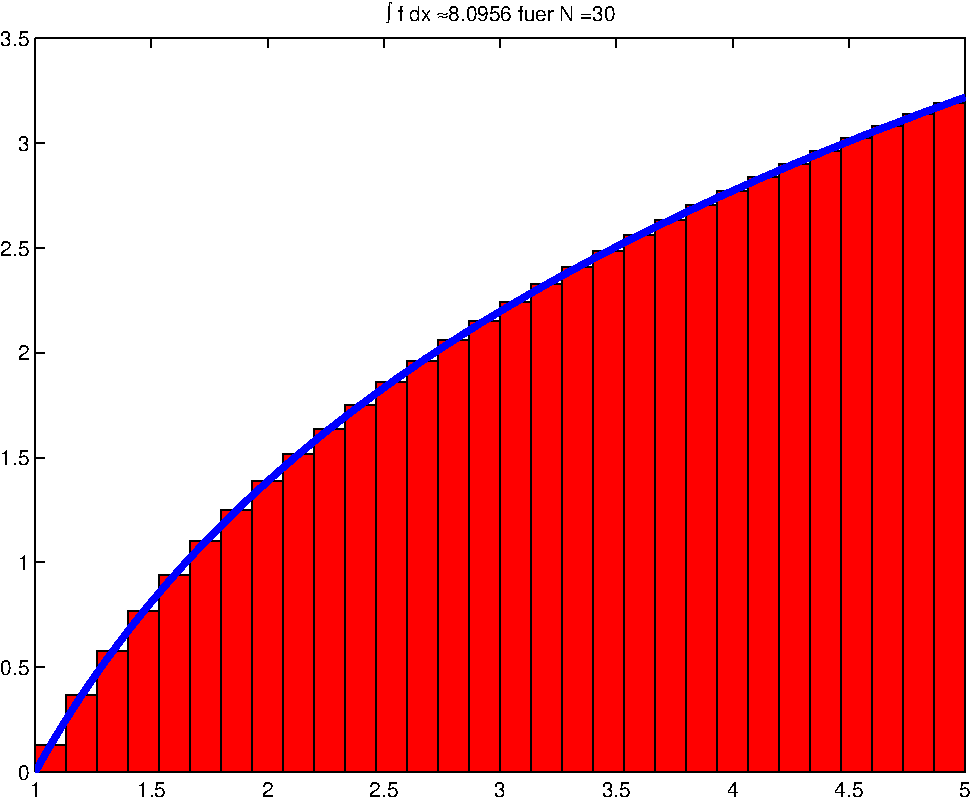
\includegraphics[width=0.8\textwidth]{./figures/plot_log}\end{center} 
\end{frame}


%
% Slide
%
\begin{frame}[fragile]\frametitle{Beispiel: Sobolevsche Mittelungsfunktion}
\[ f(x) := \left \{ \begin{array}{ll} \exp(- \frac{1}{1-\|x\|^2}), &
\|x \| <1 \\ 0, & \|x \| \geq 1 
\end{array} \right .  
\]
mit $\|x\|^2:=\sum_{i=1}^N x_i^2$, $x=(x_1, \dots x_N) \in
\mathbb{R}^N$.\\[0.5cm]

2 Versionen:
\begin{itemize}
\item eindimensionale Version
\item N-dimensionale Version
\end{itemize}
\end{frame}
%
% Slide
% TODO: python
\begin{frame}[fragile]\frametitle{Matlab: 1d-Fall}
\matinput{f_1d.m}
\end{frame}
%
% Slide
%
\begin{frame}[fragile]\frametitle{Matlab: n-dimensionaler-Fall}
\begin{matlabin}
function result = f(varargin)
% f.m     Sobolevsche Mittelungsfunktion
%         Eingabe: Matrizen x1,x2,x3,..
%         Ausgabe: Matrix result=f(x1,x2,...)
betrag = varargin{1}.^2;
for i = 2:nargin
  betrag = betrag+varargin{i}.^2;
end
dimension = size(varargin{1});
result = zeros(dimension(1),dimension(2));
for j = 1:dimension(1)
  for k = 1:dimension(2)
    if betrag(j,k) < 1
      result(j,k) = exp(-1/(1-betrag(j,k)));
    else
      result(j,k) = 0;
    end;
  end;
end;
\end{matlabin}
\end{frame}

\begin{frame}[fragile]{Python: n-dimensionaler Fall}
  \begin{pyin}
def sobnd(*args):
    """ Sobolevsche Mittelungsfunktion
    Eingabe : Matrizen x1 ,x2 ,x3 ,..
    Ausgabe : Matrix result =f(x1 ,x2 ,...)"""

    betrag = 0.
    for i in args:
        betrag += i**2
    dimension = args[0].shape
    result = zeros((dimension[0] ,dimension[1]))
    for j  in range(0,dimension[0]):
        for k in range(0,dimension[1]):
            if betrag[j,k] < 1:
                result[j,k] = exp ( -1/(1 - betrag[j,k]))
            else:
                result[j,k] = 0
    return result    
  \end{pyin}
\end{frame}

%
% Slide
%
\begin{frame}[fragile]\frametitle{Matlab: Programm zum Plotten}
\begin{matlabin}
% Eindimensionaler Plot
subplot(2,2,1),
ezplot(@f);

% Zweidimensionaler Plot
subplot(2,2,2),
ezmesh(@f);

% Zweidimensionaler Plot
subplot(2,2,3),
ezsurfc(@f);

% Zweidimensionaler Plot
subplot(2,2,4),
ezcontourf(@f);
\end{matlabin}
\end{frame}


\begin{frame}[fragile]\frametitle{Plots der Funktion}
\begin{center}
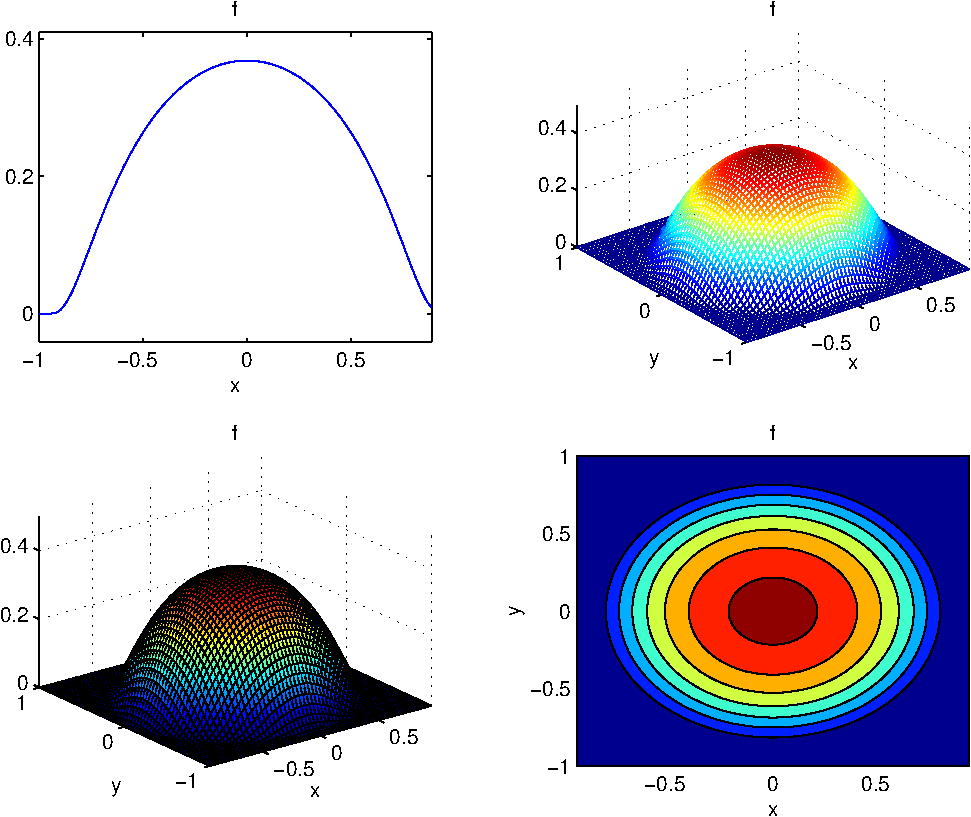
\includegraphics[width=0.8\textwidth]{./figures/plot_f}  
\end{center}
\end{frame}

% 
% Slide
% 
\begin{frame}[fragile]\frametitle{}
\centering\alert{ \imatlab{integral2(@f,50,-1.1,1.1)}}\\
\begin{center}
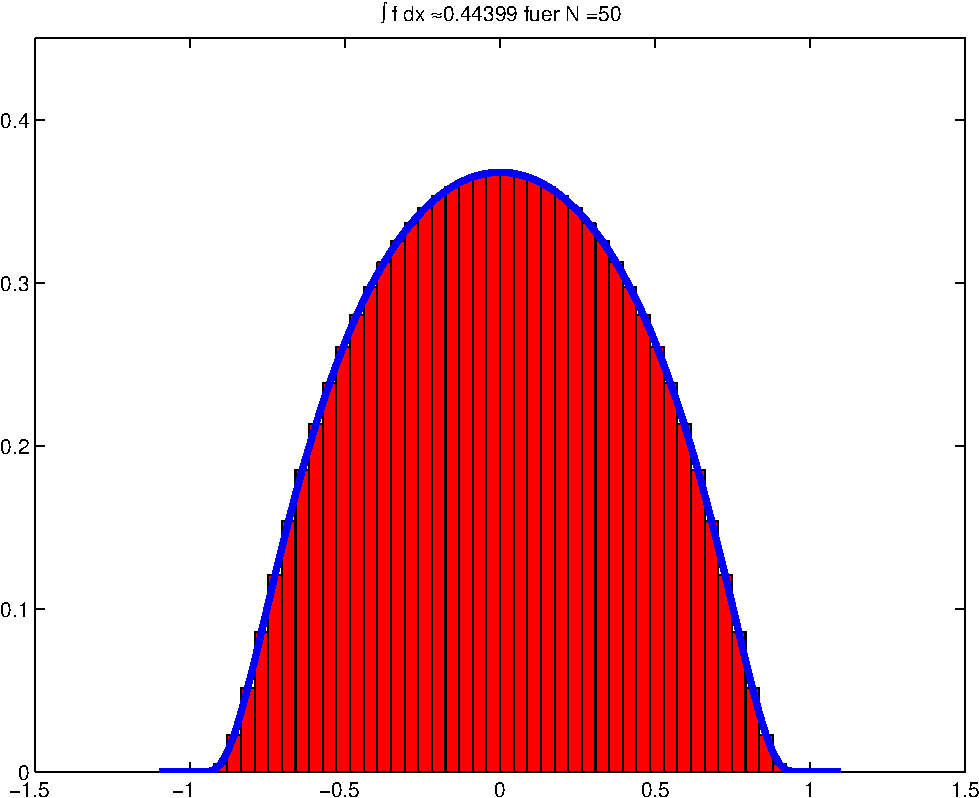
\includegraphics[width=0.8\textwidth]{./figures/plot_sobolev} 
\end{center}
\end{frame}



\section{Numerische Lineare Algebra}

\subsection{Normen}
% 
% Slide
%
\begin{frame}[fragile]\frametitle{Vektornorm}
\begin{matlabin}
norm(x,p) 
\end{matlabin}
(Default: $p=2$) 

$x=(x_1, {} \dots , x_n)$
\begin{itemize}
\item Die $p$-Norm (definiert für $p\geq 1$).
\[ \|x \|_p := \left( \sum_{i=1}^n  |x_i|^p \right)^{1/p} \] 
\item $p=\infty$  Maximum-Norm 
\[  \|x \|_\infty = \max_{i=1, \dots n} |x_i|. \]
\end{itemize}
\end{frame}
% 
% Slide
%
\begin{frame}[fragile]\frametitle{Matrixnorm}
\begin{matlabin}
norm(A,p) 
\end{matlabin}
(Default $p=2$).

Seien  $A\in \mathbb{C}^{n \times m}$ und $p \geq 1$. 
\begin{itemize}
\item $p=1$ Spaltensummennorm:
\[ 
%\| A \|_p = \sup_{x\in \mathbb{C}^m \setminus \{ 0 \}} \frac{\|Ax \|_p}{\| x \|_p}. 
\| A \|_1 = max_j \sum_{i=1}^n \abs{a_{ij}}
\]
\item $p=2$ Spektralnorm ($\lambda_{max}$: größter Eigenwert):
\[
\| A \|_2 = \sqrt{\lambda_{max} (A^H \cdot A)}
\]
\item $p=\infty$ Zeilensummennorm:
\[ 
\|A\|_\infty = \max_{1 \leq j \leq m} \sum_{i=1}^n |a_{ij}|, \quad
\]
\end{itemize} 
\end{frame}
% 
% Slide
%
\begin{frame}[fragile]\frametitle{Kondition}
Kondition einer quadratischen Matrix $A$: 
{ \[ \cond_p(A):=\|A\|_p\|A^{-1}\|_p. \] }
\vspace*{-0.8cm}
\begin{matlabin}
cond(A,p)
\end{matlabin}
(Default $p=2$)
\begin{itemize}
\item Es gilt $\cond_p(A)\geq 1$.
\item Die Kondition mißt die Empfindlichkeit der Lösung $x$ von $Ax=b$
  gegenüber  Störungen
  von $A$ und $b$.
\item Ist $\cond_p(A) >> 1$, so ist die Matrix beinahe singulär. Die Matrix ist {\it schlecht konditioniert}.
\end{itemize}
\end{frame}
% 
% Slide
%
\begin{frame}[fragile]\frametitle{Beispiele}
\begin{itemize}
\item Vektornormen für $x=(1/100) (1, 2, \dots, 100)$
\begin{matlabin}
>> x = (1:100)/100; [norm(x,1) norm(x,2) norm(x,inf)]
ans =   50.5000    5.8168    1.0000
\end{matlabin}
\item Matrixnorm für die Hilbert-Matrix $H=(\frac{1}{i+j-1})_{ij}$
\begin{matlabin}
>> H = hilb(10); [norm(H,1) norm(H,2) norm(H,inf)]
ans =    2.9290    1.7519    2.9290
\end{matlabin}
\item Kondition der Hilbert-Matrix
\begin{matlabin}
>> H = hilb(10); [cond(H,1) cond(H,2) cond(H,inf)]
ans =
   1.0e+13 *
    3.5354    1.6025    3.5354
\end{matlabin}
\end{itemize}
\end{frame}

\subsection{Lösen linearer Gleichungssyteme}
% 
% Slide 
%
\begin{frame}[fragile]\frametitle{Lineare Gleichungssysteme}
Seien $A \in \mathbb{C}^{n\times n}$ und $b \in \mathbb{C}^n$. Das
lineare Gleichungssystem 
{ \[ A x=b \]}
wird gelöst durch  
\begin{matlabin}
x=A\b
\end{matlabin}
\begin{pyin}
solve(A,b)
\end{pyin}
\textsl{Beispiel}:

\begin{matlabin}
x = ones(5,1); H = hilb(5); b = H*x; y = (H\b)'
\end{matlabin}
\begin{pyin}
x = ones((5,1)); H = hilbert(5); b = dot(H,x); y = solve(H,b)  
\end{pyin}
\begin{matlab}
y = 1.0000    1.0000    1.0000    1.0000    1.0000
\end{matlab}

\alert{Warnung:} Benutze nie
\imatlab{x=inv(A)*b}, da das Berechnen von $A^{-1}$ sehr aufwendig sein kann.
\end{frame}
% 
% Slide 
%
\begin{frame}[fragile]\frametitle{LU-Zerlegung}
{\centering  Welche Verfahren werden benutzt?}\\[0.5cm]

Meistens LU-Zerlegung von $A$ (Gaussverfahren):
\begin{itemize}
 \item obere Dreiecksmatrix $U$
 \item untere Dreiecksmatrix $L$ mit Einsen auf der Diagonalen
\end{itemize}
so dass $PA=LU$ gilt ($P$ Permutationsmatrix).

Dann wird das LGS durch Rückwärts- und Vorwärtseinsetzen gelöst
($Lz = Pb$, $Ux = z$)

\begin{matlabin}
[L,U,P]=lu(hilb(5)); norm(P*hilb(5)-L*U)
\end{matlabin}
\begin{matlab}
ans =  2.7756e-17
\end{matlab}
\end{frame}
% 
% Slide 
%
\begin{frame}[fragile]\frametitle{Inverse, Pseudoinverse, Determinante}
\begin{itemize}
\item Berechnung der Inversen
\begin{matlabin}
inv(A)
\end{matlabin}
\item (Moore-Penrose) Pseudoinverse: 
Sei $A$ singulär, Bestimme $X$ so dass 
\[ A X A=A,  X A X =X,  (X A)^* =X A,  (A X )^* = A X \]
\begin{matlabin}
>> pinv(ones(3,3))
ans =
    0.1111    0.1111    0.1111
    0.1111    0.1111    0.1111
    0.1111    0.1111    0.1111
\end{matlabin}
\item Berechnung der Determinante
\begin{matlabin}
det(A)
\end{matlabin}
\end{itemize}
\end{frame}

\subsection{Anwendung: Zwei-Punkt-Randwert-Aufgabe}
%
% Slide
%
\begin{frame}[fragile]\frametitle{Zwei-Punkt-Randwert-Aufgabe}

Suche eine Funktion 
\begin{equation*}
u:[0,1] \quad \rightarrow \quad \mathbb{R}, 
\end{equation*}
so dass 
\begin{eqnarray*}
-u''(x) & = & e^x, \quad x \in (0,1)\\
u(0) & = & u(1) =0
\end{eqnarray*}
\alert{Problem:} Es kann i.A. keine geschlossene
Lösungsdarstellung angegeben werden. \\ %Wieso ->relativ offensichtlich.. (wegen randbedingungen)

\alert{Ausweg:} Approximation der Lösung. 
\end{frame}
%
% Slide: 
%
\begin{frame}[fragile]\frametitle{Finite Differenzen Verfahren}

\begin{itemize}
 \item Diskretisierung: $0=x_0 < \dots < x_{n}=1$ mit $x_i=\frac{i}{n}$
\item Differenzenquotient: 
\[ u''(x_i) \sim \frac{u(x_{i-1}) - 2 u(x_i) + u(x_{i+1})}{ 
  h^2}, \quad h:=\frac{1}{n} \]
\item Einsetzen in $-u''(x)=e^x$ ergibt 
\[ -u(x_{i-1}) + 2 u(x_i) - u(x_{i+1}) =  h^2 e^{x_i}, \quad
i=1,\dots ,n-1 \] 
Randbedingungen $\Rightarrow $ $u(x_0)=u(x_n)=0$.
\item $\Rightarrow$ Lineares Gleichungssystem für 
$u(x_1), \dots ,u(x_{n-1})$.
\end{itemize}

\end{frame}

%
% Slide: 
%
\begin{frame}[fragile]\frametitle{Diskretes Problem}

Setze $z=(z_1,\dots ,z_{n-1})^t=(u(x_1), \dots ,u(x_{n-1}))^t$. \\

Löse das Gleichungssystem  $Az=F$  mit 
\[ A:= 
\left( \begin{array} {ccccccc}
 2 & -1 &  & &   0 \\
-1 & 2  & -1 &    & \\ 
   & \ddots & \ddots & \ddots   &\\
   & &  -1 & 2  & -1  \\ 
0 &  &    & -1 & 2 \\
\end{array} \right), \  F:=
h^2 \left( \begin{array}{c} e^\frac{1}{n}\\   \vdots \\ e^\frac{n-1}{n}
\end{array} \right) .
\] 
\end{frame}
%
% Slide: 
%
\begin{frame}[fragile]\frametitle{Implementation für $n=21$}
\begin{itemize}
\item Zerlegung des Intervalls $[0,1]$
\begin{matlabin}
x = 0:(1/n):1
\end{matlabin}
\item Eleminieren der Randpunkte
\begin{matlabin}
x_i = x(2:n)
\end{matlabin}
\item Erzeugen der Matrix $A$ (Übungsaufgabe)
\end{itemize}
\end{frame}
%
% Slide: 
%
\begin{frame}[fragile]\frametitle{Lösung für $n=21$}
\begin{itemize}
\item Berechnen der rechten Seite:
\begin{matlabin}
F = (1/21)^2*transpose(exp(x_i));
\end{matlabin}
\item Lösen des linearen Gls.\\
\begin{matlabin}
z_i = A\F;
\end{matlabin}
\item Zufügen der Werte am Rand
\begin{matlabin}
z = [0; z_i;0];
\end{matlabin}
\end{itemize}
\end{frame}
%
% Slide: 
%
\begin{frame}[fragile]\frametitle{Lösung für $n=21$}
\begin{columns}[c]
\column{0.48\textwidth}
\begin{matlabin}[basicstyle=\tiny]
plot(x,z,'r*','MarkerSize',8)
\end{matlabin}
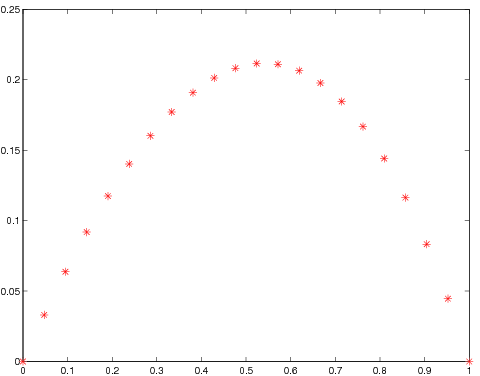
\includegraphics[width=\textwidth]{figures/bild1_27_10}

\column{0.48\textwidth}
\begin{matlabin}[basicstyle=\tiny]
plot(x,z,'r*-','LineWidth',3,'MarkerSize',8)
\end{matlabin}%
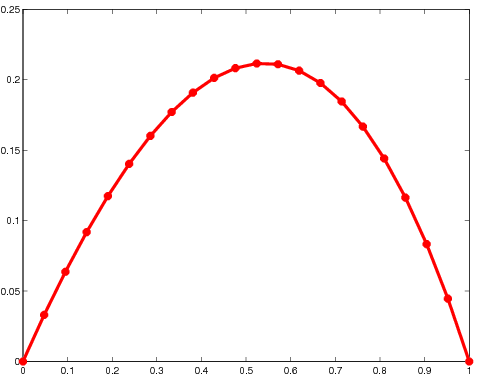
\includegraphics[width=\textwidth]{figures/bild2_27_10}
\end{columns}
\end{frame}


\subsection{Bestimmung von Eigenwerten}
% 
% Slide 
%
\begin{frame}[fragile]\frametitle{Eigenwerte}
\begin{block}{Eigenwert}
Sei $A \in \mathbb{C}^{n \times n}$. $\lambda \in \mathbb{C}$ ist
Eigenwert von $A$, falls ein Vektor $x \in \mathbb{C}^n$ ungleich $0$ existiert, so
dass  $Ax = \lambda x$ gilt. $x$ heißt Eigenvektor.  
\end{block}

\begin{itemize}
\item 
  \begin{matlabin}
x=eig(A)
  \end{matlabin}
  berechnet die Eigenwerte von $A$ und schreibt
  sie in den Vektor $x$.
\item
  \begin{matlabin}
[V,D]=eig(A)
  \end{matlabin}
  $D$ ist eine Diagonalmatrix mit den Eigenwerten auf der
  Diagonalen. Die Spalten von $V$ bilden die zugehörigen Eigenvektoren. 
\end{itemize}
\end{frame}
% 
% Slide 
%
\begin{frame}[fragile]\frametitle{Weitere Zerlegungen}
\begin{itemize}
\item \alert{QR-Zerlegung}: 
  \begin{matlabin}
[Q,R]=qr(A)
  \end{matlabin}
  $m \times n$- Matrix $A$ eine Zerlegung { $A=QR$} erzeugt,
  ($Q$ eine unitäre $m \times m$-Matrix, $R$ eine obere $m \times n$ Dreiecksmatrix).
%Die QR-Zerlegung spielt in vielen Verfahren der numerischen Mathematik  eine wichtige Rolle, 
%beispielsweise um eine orthogonale oder unitäre Basis zu bestimmen oder um lineare Ausgleichsprobleme 
%zu behandeln. 
%QR-Algorithmus zur Berechnung aller Eigenwerte einer Matrix.
\item \alert{Singulärwertzerlegung}: 
  \begin{matlabin}
[U,S,V]=svd(A)
  \end{matlabin}
  { $A=U \Sigma V^*$}. 
  ($\Sigma \subset \mathbb{C}^{m \times n}$ eine Diagonalmatrix \\
  $U \subset \mathbb{C}^{m \times m}$, $V \subset  \mathbb{C}^{n \times n}$ unitäre Matrizen). 
%Dieses Verfahren wird insbesondere in der numerischen Mathematik verwendet. Dort lassen sich beispielsweise quasisinguläre 
%lineare Gleichungssysteme im Rahmen rechentechnischer Genauigkeiten passabel lösen.
%In der Statistik ist die SVD der rechnerische Kern der Hauptkomponentenanalyse, dort auch Karhunen-Loève-Transformation genannt.
%Einige moderne Bildkompressionsverfahren beruhen auf einem Algorithmus, der das Bild (=Matrix aus Farbwerten) in eine SVD überführt 
%und anschließend nur die stark von null verschieden Elemente der Matrix Σ berücksichtigt und dann die zur Rückgewinnung der Matrix 
%erforderlichen Vektoren sowie die verbliebenen Diagonalelemente speichert. Besonders effektiv ist diese Kompression bei 
%bestimmten rechteckigen Mustern und natürlich, je größer (und je quadratischer) das Bild ist. Dies ist eine mögliche Anwendung 
%von Modellreduktion. Das Weglassen von kleinen Singulärwerten ist ein verlustbehaftetes Modellreduktionsverfahren.

\item \alert{Cholesky-Zerlegung}: 
  \begin{matlabin}
R=chol(A) | R=cholesky(A)
  \end{matlabin}
  { $A=R^*R$} zu einer hermiteschen, positiv definiten Matrix
  $A$ ($R$ ist eine obere Dreiecksmatrix mit reellen, positiven
  Diagonalelementen). 
\end{itemize}
%Eine Matrix A heißt hermitesch (nach Charles Hermite) oder selbstadjungiert genau dann, wenn sie gleich ihrer 
%(hermitesch) Adjungierten A * , also gleich der transponierten und komplex konjugierten Matrix ist. D. h.

%positiv definit, 	falls x^T Ax > 0

%Die Cholesky-Zerlegung kann auch zur Gewinnung eines Vorkonditionierungsverfahrens für lineare Gleichungssysteme mit 
%positiv definiter Matrix benutzt werden; zu diesem Zweck gibt es speziell die Variante der unvollständigen Cholesky-Zerlegung 
%sowie der modifizierten unvollständigen Cholesky-Zerlegung.
% determinante
% test ob es eine positiv definite matrix ist
\end{frame}
% 
% Slide 
%
\begin{frame}[fragile]\frametitle{Bemerkungen}
\begin{itemize}
\item LGS können auch mit Hilfe iterativer Verfahren gelöst werden:
\begin{itemize}
 \item \imatlab{gmres} (generalized minimum residual)
 \item \imatlab{pcg}| \isage{cg} (preconditioned conjugate gradient)
 \item \imatlab{bicgstab} (biconjugate gradients stabilized)
 \item Jacobi
 \item overrelaxed Gauss-Seidel (SOR)
\item \ldots
\end{itemize}
%\item $A\in \mathbb{C}^{n \times m}$, $n \neq m$ bei \imatlab{A\\b}:
%\begin{itemize}
%\item $n>m$ (überbestimmter Fall): Least-Square Lösung, d.h. der Ausdruck
%  \imatlab{norm(A*x-b)} wird minimiert. 
%\item $n<m$ (unterbestimmter Fall): Grundlösung. 
%\end{itemize}
\end{itemize}
\end{frame}


\section{D\"unnbesetzte Matrizen}

% 
% Slide 
%
\begin{frame}[fragile]\frametitle{D\"unnbesetzte Matrizen}
\begin{itemize}
\item Bei {\it D\"unnbesetzten Matrizen} ({\it sparse matrices}) sind
  fast alle Eintr\"age $0$.
\item In vielen Anwendungen, z.B. bei der Diskretisierung von
  Differentialgleichungen oder in der Graphentheorie, treten sehr
  grosse, d\"unnbesetzte  Matrizen auf.
\item eigener Datentyp, der zu
  jedem Nichtnullelement der Matrix, die zugeh\"orige Zeile und Spalte
  speichert.    
\end{itemize}
\end{frame}
% 
% Slide 
%
\begin{frame}[fragile]\frametitle{}
\begin{itemize}
\item Erzeugung einer d\"unnbesetzten Matrix
  der Gr\"osse $n \times m$. Alle Eintr\"age sind $0$.
\begin{matlabin}
sparse(n,m) 
\end{matlabin}
\begin{pyin}
sparse.csr_matrix((n,m))
\end{pyin}

\item Konvertierung der dichtbesetzten Matrix
  $A$ in eine d\"unnbesetzte Matrix.
\begin{matlabin}
sparse(A)
\end{matlabin}
\begin{pyin}
sparse.csr_matrix(A)
\end{pyin}

\item Die Struktur der Matrix $A$ visualisieren.
\begin{matlabin}
spy(A)
\end{matlabin}

\item Die meisten Standardoperationen funktionieren auch mit
  d\"unnbesetzten Matrizen.  
\end{itemize}
\end{frame}
% 
% Slide 
%
\begin{frame}[fragile]\frametitle{Beispiel}
\begin{matlabin}
A = 2*diag(ones(10,1),0) ...
       - diag(ones(9,1),-1) ...
       - diag(ones(9,1),1);
B = sparse(A)
\end{matlabin}
\begin{matlab}
B =   (1,1)        2
      (2,1)       -1
      (1,2)       -1
      (2,2)        2
\end{matlab}
\begin{pyin}
import scipy.sparse as sparse
A = 2*diag(ones((10,)),0)+diag(ones((9,)),-1)+diag(ones((9,)),1)
sparse.csr_matrix(A)
\end{pyin}
\begin{pyout}
<10x10 sparse matrix of type '<type 'numpy.float64'>'
  with 28 stored elements in Compressed Sparse Row format>
\end{pyout}
%\begin{matlab}
%  Name      Size           Bytes  Class
%  A        10x10             800  double array
%  B        10x10             380  sparse array
%\end{matlab}
\end{frame}
% 
% Slide 
%
\begin{frame}[fragile]\frametitle{Dichte und d\"unnbesetzte Matrizen}
\begin{itemize}
\item Konvertierung der d\"unnbesetzten Matrix $A$ in eine dichtbesetzte Matrix $B$ .
\begin{matlabin}
B = full(A)
\end{matlabin}
\begin{pyin}
A.todense()  
\end{pyin}
\item Bei bin\"aren Operationen, z.B. $A+B$ oder $A*B$ ist das Ergebnis
  bei d\"unnbesetzten Matrizen $A$ und $B$ wieder eine d\"unnbesetzte
  Matrix. \\Ist eine der Matrizen dichtbesetzt, so ist auch das Ergebnis
  dichtbesetzt. 
\item Berechnung der $k$ betragsm\"a{\ss}ig  gr\"ossten Eigenwerte (Default: $k=6$):
\begin{matlabin}
eigs(A,k) 
\end{matlabin}
\begin{pyin}
scipy.sparse.linalg.eigs(A,k)
\end{pyin}
\end{itemize}
\end{frame}
% 
% Slide 
%
\begin{frame}[fragile]\frametitle{}
\begin{itemize}
\item Norm- und Konditionsberechnung:
\begin{matlabin}
normest(<A>) , condest(<A>)
\end{matlabin}
\begin{pyin}
norm(<A>), cond(<A>)  
\end{pyin}

\item Alle iterativen Verfahren funktionieren auch mit d\"unnbesetzten
  Matrizen (oder haben eine spezielle Version) 
\item Indizes aller Zeilen und Spalten erhalten, in denen Nichtnullelemente stehen: 
\begin{matlabin}
[I,J] = find(X)
\end{matlabin}
\item Eine \"Ubesicht aller Funktionen f\"ur d\"unnbesetzte Matrizen erh\"alt
  man durch \alert{ \imatlab{help sparfun}| \isage{scipy.sparse}}.  
\end{itemize}
\end{frame}

\end{document}
 

